\documentclass[aps,rmp,preprint,amsmath,amssymb,graphicx,longbibliography]{revtex4-1}

\usepackage{bm}
\usepackage{graphicx}
\usepackage{epstopdf}
\usepackage{wrapfig}
\usepackage{array} 
\usepackage{listings}
\usepackage[para,online,flushleft]{threeparttablex}
\usepackage{booktabs,dcolumn}
\usepackage{color}

 

\usepackage{textpos}
\usepackage{booktabs}
\usepackage{multirow,bigdelim}
\usepackage{float}

\usepackage{upgreek} %upalpha in Saxena2021 Reference

\usepackage[utf8]{inputenc}
\usepackage{hyperref}
\hypersetup{breaklinks=true,colorlinks=true,linkcolor=blue,citecolor=blue,filecolor=magenta,urlcolor=blue}

\usepackage{xcolor}
\newcommand{\contrib}[1]{\textcolor{red}{#1}}
\newcommand{\comment}[1]{\textcolor{blue}{#1}}
\newcommand{\WN}[1]{{\color{red} #1}}

\makeatletter
\def\@bibdataout@aps{%
\immediate\write\@bibdataout{%
@CONTROL{%
apsrev41Control%
\longbibliography@sw{%
    ,author="08",editor="1",pages="1",title="0",year="1"%
    }{%
    ,author="08",editor="1",pages="1",title="",year="1"%
    }%
  }%
}%
\if@filesw \immediate \write \@auxout {\string \citation {apsrev41Control}}\fi
}
\makeatother

\begin{document}

\title{\underline{Computational Physics and Quantum Technologies}; a new Bachelor of Science program  at the Department of Physics, University of Oslo}

\author{Morten Hjorth-Jensen and Anders Malthe-Sørenssen}
\affiliation{Department of Physics and Center for Computing in Science Education, University of Oslo}


\begin{abstract}
We propose to establish, with {\em startup Fall semester 2023}, a new bachelor/undergraduate program in {\bf Computational Physics and Quantum Technologies, (CompPhysQuantum)}  at the University of Oslo, hosted by the Department of Physics. 
\end{abstract}
\maketitle
\section{Introduction}

Computational physics, computational science  and data science play a central role in scientific investigations and are central to innovation in most domains of our lives. These fields underpin the majority of today's technological, economic and societal feats. We have entered an era in which huge amounts of data offer enormous opportunities, but only to those who are able to harness them. The 3rd industrial revolution will alter significantly the demands on the workforce. In particular, the developments taking place in quantum technologies and quantum information systems (QIS) together with artificial intelligence (AI) and machine learning (ML) are expected to play a significant role in technology developments and innovations, and for potential discoveries in Physics.

Artificial intelligence and ML techniques\footnote{Artificial intelligence is built upon integrated machine learning algorithms, which in turn are fundamentally rooted in optimization and statistical learning.} have in the last years gained considerable traction in scientific discovery. In particular, applications and techniques for so-called {\em fast} ML, that is high-performance ML methods applied to real time experimental data processing, hold great promise for enhancing scientific discoveries in many different disciplines \cite{deiana2021}. 
These developments cover a broad mix of rapidly evolving  fields, from the development of ML techniques to computer and hardware architectures. For our research in for example particle and nuclear physics, which cover a huge range of energy and length scales, spanning from our smallest constituents to the physics of dense astronomical objects like supernovae and neutron stars, AI and ML techniques offer possibilities for new discoveries and deeper insights about the physics of atomic nuclei, elementary particles and dense matter. Similarly, ML algorithms are widely applied  in condensed matter physics, materials science and nanotechnology \cite{Schleder2019} and in many other  fields in physics and the physical sciences.

In addition, the recent developments in quantum information systems and technologies offer the possibility to address some of the most challenging large-scale problems, whether they are represented by complicated interacting quantum mechanical systems or classical systems.
Originally proposed by Feynman, the efficient
simulation of for example quantum systems by other, more controllable quantum
systems formed the basis for modern constructions of quantum
computation.  
Many algorithmic and theoretical advances have followed since the
initial work in this area and with recent developments in quantum computing
hardware there is an additional drive to identify early practical problems on
which these devices might demonstrate an advantage. In addition to theoretical activities conducted at the Department of Physics (mainly at the Center for Computing in Science Education (CCSE) and the condensed matter group), there is a growing interest to study candidate systems for making quantum hardware. In particular, so-called point defects in semiconductors are pursued by experimenters at the center for Materials Science. 
With these broad list of activities at the department of physics, there is a huge potential to prepare the ground for educating physicists with the theoretical and experimental background needed for the 21st century. There is also a great interest in candidates with such a background, knowledge, skills and competences in industry and the public sector.
Establishing such an educational program will be unique in Norway and has the potential to attract excellent students.  



\section{Short background and Motivation}

Computational physics plays a central role in the above mentioned   developments. 
Computations are simply indispensable. 
At the department of physics of the university of Oslo this is reflected in the extremely popular study direction Computational Physics of the master of science program Computational Science. This program has over the last two decades recruited many excellent students, resulting in highly attractive candidates in academia and in industry  and the public sector. A large fraction of these students have specialized either in artificial intelligence and machine learning and/or in quantum information systems.  The large  majority of the these students have job offers at least one year before completing their MSc theses. Furthermore, with recent advances in quantum technologies, there is a strong potential for new developments in the fields of nanotechnology and materials science, with the possibilities to develop new experimental activities. 

The rationale behind proposing a new BSc program in computational physics and quantum technologies (QT) is:
\begin{enumerate}
    \item To attract at an earlier stage new students with an explicit interest in QIS, QT and AI and ML in physics. 
    \item To enhance the recruitment to fields in physics which are in high demand for students and candidates with an expertise in computations, QIS, QT, AI and ML. We expect high demands from both the private sector and the public sector for candidates with these competences, insights and skills.
    \item Candidates with such a background will be of great importance for new scientific discoveries and technological innovations. At the department of physics of the university of Oslo there are several research directions whose scientific activities will benefit at large from candidates with such a background, spanning from fast ML for new discoveries to the development of QTs.   
\end{enumerate}


\section{Structure of Program and Courses}

In developing such a program, we firmly believe that 
the Center for Computing in Science Education (CCSE) at the university of Oslo (UiO) should be the entity which provides the pedagogical resources. It has the needed research experience
on how to design curricula so that students develop deep knowledge that is connected and useful.
The figure here, inspired by the QuSTEAM project in the USA \url{https://qusteam.org/}
shows how one can link educational developments by involving various stakeholders from academia, industry and national laboratories. 
\begin{figure*}[!htb]
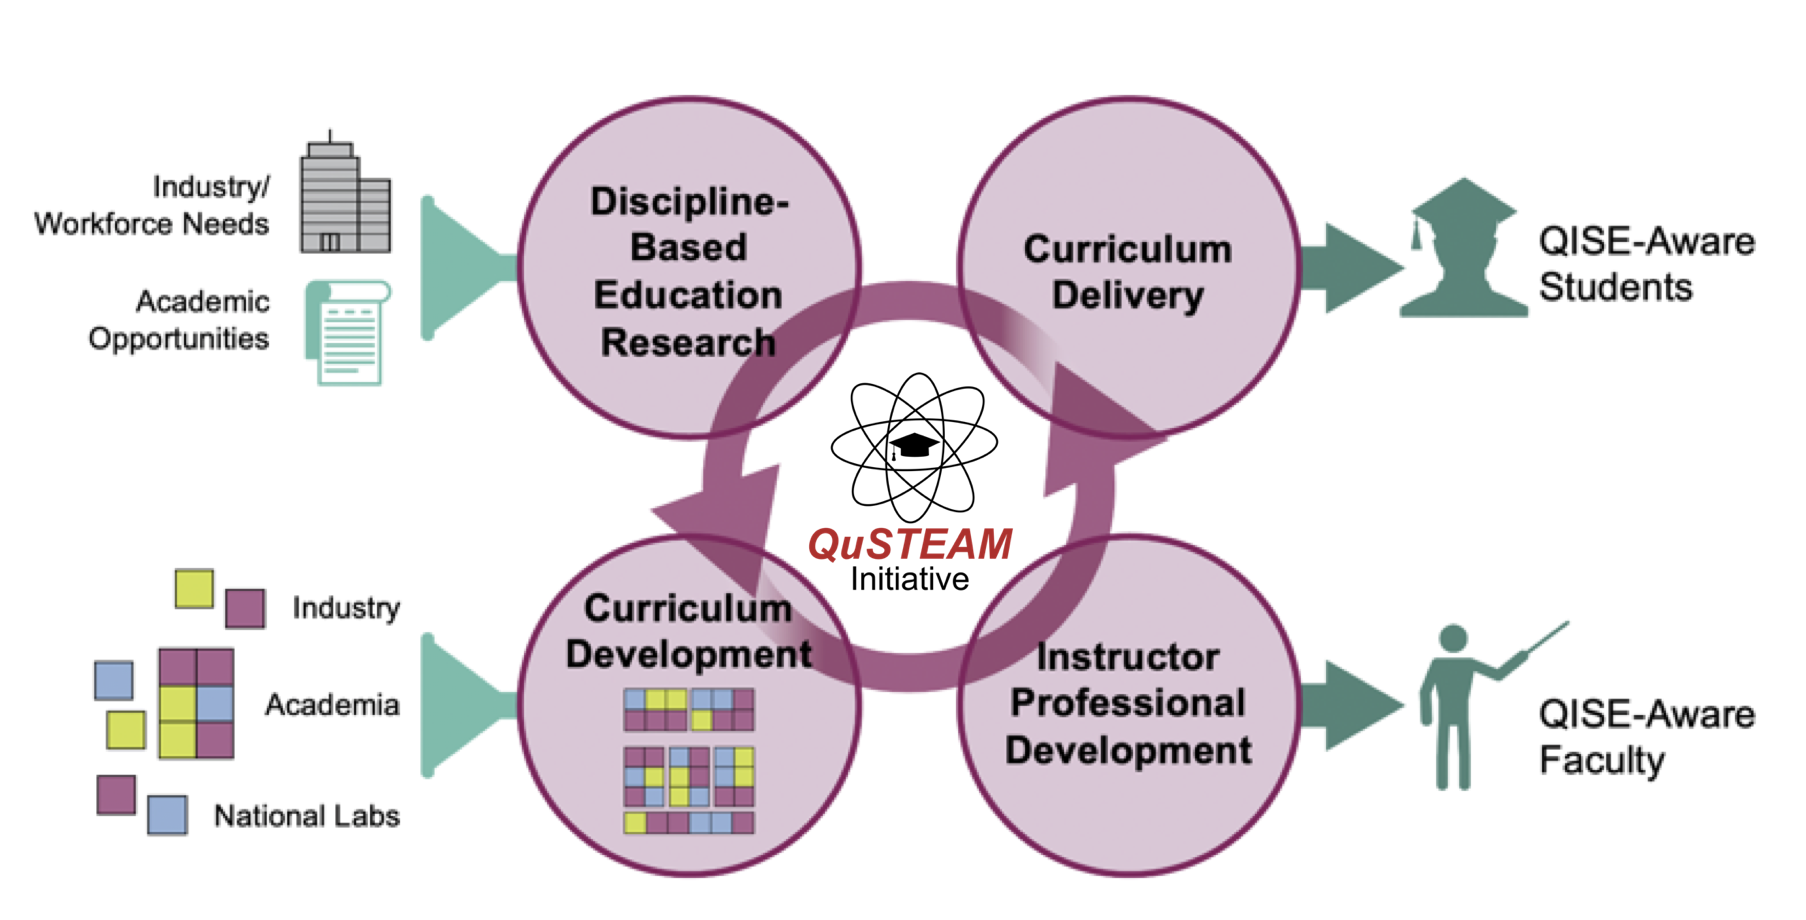
\includegraphics[width=1.0\linewidth]{qusteam.png}
\end{figure*}


The reason why we believe the CCSE should be involved in planning this BSc program is that it has the necessary expertise to address several issues, such as
\begin{enumerate}
    \item  Lots of conceptual learning: superposition, entanglement, QIS and QT, etc. 
    \item Connecting statistics and mathematics with ML methods
    \item Linking ML algorithms with quantum ML.
\item Coding is indispensable. This is a central reason why the CCSE should be involved.
\item Experience with teamwork, project management, and communication are important and highly valued.
\item  Experience with engagement with industry, public sector and priority to diversity through the Computational Science program and other activities at the CCSE
\item  Mentorship should begin the moment students enroll. The experiences with the Computational Science program developed at the CCSE will be of great value, as the activities of the KURT center.
\end{enumerate}

The program aims at addressing future societal needs, such as the  needs for specialized candidates (PhDs, postdocs), but also the needs of  people with a broad overview of what is possible in  QIS and QT. There are  not enough potential employees in AI, ML, QIS and QT. It is a supply gap, not a skills gap.

A BSc degree  with specialization  is thus a good place to start. Linking this with the Computational Science program and the study directions Computational physics and Computational materials science, will offer our various research fields top candidates as well as pointing to new research directions. 

\subsection{Paths in the BSc program}

The program proposes two possible directions in the last year
\begin{enumerate}
    \item Quantum information systems and quantum technologies
    \item Artificial intelligence and machine learning in physics
\end{enumerate}

There are several existing courses which can be included in this program. There are also courses which need to be established. At the CCSE we have the research and educational expertise to establish two to three new courses in these directions.
A separate application for establishing these courses follows. The additional courses we propose are (these are suggestions and codes are tentative) listed here. Note that we propose thee courses as cloned courses. We may consider extensions of these codes in order to offer PhD variants as well.



\begin{enumerate}
    \item \color{red} Classical and quantum laboratory, needs to be established, perhaps by researchers at the Center of Materials Science (LENS group), FYS2440
    \item Quantum computing and software (CCSE), FYS3440/FYS4440
    \item Quantum hardware, FYS3445/FYS4445, needs to be established, perhaps by researchers at the Center of Materials Science (LENS group)
    \item Quantum computing and quantum machine learning, FYS3446/FYS4446 (cloned course, developed by CCSE)
    \item Advanced machine learning and data analysis for the physical sciences, FYS3447/FYS4447 (developed by CCSE)
\end{enumerate}

The last three course are elective ones for the last semester of study. Some of these courses can also be split into modules a 5 ECTS or 7.5 ECTS.
The first year is identical with the BSc program Physics and Astronomy.

\begin{table}
 \caption{Basic structure of the program. Courses marked in red are among the new courses listed in the text.}
    \centering
    \begin{tabular}{|c|c|c|c|} \hline
    First Semester & MAT1100 &  IN1900   & FYS11XX  \\ \hline 
    Second Semester & MAT1110 & FYS12XX  & FYS13XX \\ \hline
    Third Semester & MAT1120 &   FYS1120  &  FYS3150 (Comp Phys)\\ \hline
    Fourth Semester & FYS2130 & FYS2140    & \color{red} {FYS2440}/STK2100 \\ \hline       
    Fifth Semester & FYS2160 & FYS3110     & \color{red}Elective/FYS-STK3155 \\ \hline
    Sixth Semester & \color{red} Elective/EX-PHIL & \color{red} Elective    & \color{red} Elective \\ \hline
   ECTS & 10 &  10   &  10  \\ \hline    
    \end{tabular}
\end{table}


\bibliography{References}


\end{document}

